\documentclass[11pt,letterpaper]{article}

\usepackage[utf8]{inputenc}
\usepackage[T1]{fontenc}
\usepackage[spanish,es-tabla]{babel}
\usepackage{amsmath,amssymb,amsfonts}
\usepackage{geometry}
\usepackage{graphicx}
\usepackage{booktabs}
\usepackage{array}
\usepackage{multirow}
\usepackage{float}
\usepackage{caption}
\usepackage{subcaption}
\usepackage{hyperref}
\usepackage{xcolor}
\usepackage{fancyhdr}

\geometry{margin=2.3cm}
\graphicspath{{../figuras/}{figuras/}{./}}

\hypersetup{
    colorlinks=true,
    linkcolor=blue!70!black,
    urlcolor=blue!70!black,
    citecolor=blue!70!black
}

\pagestyle{fancy}
\fancyhf{}
\lhead{\small Cálculo Computacional --- Tarea 3: Interpolación}
\rhead{\small Maria Laura Gutierrez Castillo}
\cfoot{\thepage}

\begin{document}

% ==================== PORTADA ====================
\begin{titlepage}
    \centering
    {\large \textbf{UNIVERSIDAD DE CARABOBO}}\\[0.15cm]
    {\large \textbf{FACULTAD EXPERIMENTAL DE CIENCIAS Y TECNOLOGÍA (FACYT)}}\\[0.15cm]
    {\normalsize Departamento de Computación --- Asignatura: Cálculo Computacional}\\[2.2cm]

    \rule{\linewidth}{0.5mm}\\[0.4cm]
    {\LARGE \textbf{Tarea 3: Interpolación Polinómica y Splines Cúbicos Naturales}}\\[0.3cm]
    {\large Implementación Numérica, Análisis del Fenómeno de Runge y Reconstrucción Paramétrica de Curvas Planas}\\[0.2cm]
    \rule{\linewidth}{0.5mm}\\[2.0cm]

    \begin{flushleft}
        \hspace{2.2cm}\textbf{Autora:} Maria Laura Gutierrez Castillo \\
        \hspace{2.2cm}\textbf{Cédula de Identidad:} V-23.424.597 \\
        \hspace{2.2cm}\textbf{Parámetro $d$ (último dígito):} $d = 7$ \\
        \hspace{2.2cm}\textbf{Intervalo de estudio:} $[-(d+5),\, d+5] = [-12,\, 12]$ \\
        \hspace{2.2cm}\textbf{Lenguaje y herramientas:} Python 3, NumPy, Matplotlib
    \end{flushleft}

    \vfill
    {\normalsize Bárbula, Noviembre de 2026}
\end{titlepage}

\tableofcontents
\newpage

% ==================== MARCO METODOLÓGICO ====================
\section{Fundamentos Matemáticos y Algoritmos Implementados}

Para abordar los cuatro problemas propuestos se implementaron dos esquemas clásicos de interpolación numérica en Python sin utilizar rutinas de caja negra:

\subsection{Interpolación Polinómica de Newton (Diferencias Divididas)}
Dados $n+1$ nodos distintos $(x_0, y_0), (x_1, y_1), \dots, (x_n, y_n)$, el único polinomio $P_n(x)$ de grado a lo sumo $n$ que satisface $P_n(x_i) = y_i$ se expresa en la forma progresiva de Newton:
\begin{equation}
    P_n(x) = c_{0,0} + c_{0,1}(x - x_0) + c_{0,2}(x - x_0)(x - x_1) + \dots + c_{0,n}\prod_{k=0}^{n-1}(x - x_k),
\end{equation}
donde los coeficientes $c_{0,j} = f[x_0, x_1, \dots, x_j]$ se obtienen recursivamente mediante la tabla de diferencias divididas:
\begin{equation}
    f[x_i] = y_i, \qquad f[x_i, \dots, x_{i+j}] = \frac{f[x_{i+1}, \dots, x_{i+j}] - f[x_i, \dots, x_{i+j-1}]}{x_{i+j} - x_i}.
\end{equation}
La evaluación numérica en un punto $x$ se efectúa mediante el esquema anidado tipo Horner en $\mathcal{O}(n)$ operaciones aritméticas, reduciendo errores de redondeo y evitando el cálculo explícito de potencias elevadas.

\subsection{Spline Cúbico Natural (Algoritmo 3.4 de Burden \& Faires)}
Dado un conjunto de nodos ordenados $x_0 < x_1 < \dots < x_n$ con longitudes de subintervalo $h_j = x_{j+1} - x_j$, un spline cúbico natural $S(x)$ es una función definida a trozos por polinomios cúbicos
\begin{equation}
    S_j(x) = a_j + b_j(x - x_j) + c_j(x - x_j)^2 + d_j(x - x_j)^3, \qquad x \in [x_j, x_{j+1}], \quad j = 0, \dots, n-1,
\end{equation}
que pertenece a $C^2[x_0, x_n]$ (continuidad de $S$, $S'$ y $S''$ en los nodos interiores) y verifica las condiciones de frontera natural $S''(x_0) = S''(x_n) = 0$. El sistema tridiagonal estrictamente diagonal dominante asociado a las segundas derivadas ($c_0 = c_n = 0$) se resuelve en tiempo lineal $\mathcal{O}(n)$ mediante factorización de Crout.

% ==================== PROBLEMA 1 ====================
\section{Problema 1: Interpolación de Newton sobre los Dígitos de la Cédula}

\subsection{Planteamiento y Coeficientes Obtenidos}
A partir de los $8$ dígitos de la cédula de identidad \textbf{23.424.597}, se construye el conjunto de $8$ nodos $(x_i, y_i) = (i, d_i)$ para $i = 0, 1, \dots, 7$, generando un polinomio interpolante $P_7(x)$ de grado $7$.

\begin{table}[H]
    \centering
    \caption{Nodos $(x_i, d_i)$ de la cédula V-23.424.597 y coeficientes $c_{0,i}$ del polinomio de Newton $P_7(x)$.}
    \label{tab:p1_cedula}
    \begin{tabular}{cccc}
        \toprule
        Índice $i$ & Nodo $x_i$ & Dígito $y_i = d_i$ & Coeficiente $c_{0,i}$ \\
        \midrule
        $0$ & $0$ & $2$ & $+2.0000000000$ \\
        $1$ & $1$ & $3$ & $+1.0000000000$ \\
        $2$ & $2$ & $4$ & $+0.0000000000$ \\
        $3$ & $3$ & $2$ & $-0.5000000000$ \\
        $4$ & $4$ & $4$ & $+0.4166666667$ \\
        $5$ & $5$ & $5$ & $-0.1833333333$ \\
        $6$ & $6$ & $9$ & $+0.0597222222$ \\
        $7$ & $7$ & $7$ & $-0.0170634921$ \\
        \bottomrule
    \end{tabular}
\end{table}

De los valores de la Tabla~\ref{tab:p1_cedula} se observa que $c_{0,2} = 0$ debido a que los tres primeros puntos $(0,2)$, $(1,3)$ y $(2,4)$ son colineales con pendiente unitaria. El polinomio explícito resultante en base de Newton es:
\begin{align}
    P_7(x) &= 2 + x - 0.5\,x(x-1)(x-2) + 0.4166666667\prod_{k=0}^{3}(x-k) \nonumber\\
           &\quad - 0.1833333333\prod_{k=0}^{4}(x-k) + 0.0597222222\prod_{k=0}^{5}(x-k) - 0.0170634921\prod_{k=0}^{6}(x-k).
\end{align}

\subsection{Comportamiento Fuera del Rango de Interpolación}
El polinomio se evaluó sobre $200$ puntos equiespaciados en el intervalo extendido $[-2, 9]$. Como se aprecia en la Figura~\ref{fig:p1_cedula}, dentro de $[0, 7]$ la curva pasa exactamente por todos los dígitos. Sin embargo, en las regiones de extrapolación $[-2, 0)$ y $(7, 9]$, el término dominante $-0.0170634921\,x^7$ provoca un crecimiento extremadamente pronunciado hacia $+\infty$ a la izquierda de $x=0$ y una caída abrupta hacia $-\infty$ a la derecha de $x=7$. Esto evidencia la inestabilidad inherente a la extrapolación con polinomios de grado alto.

\begin{figure}[H]
    \centering
    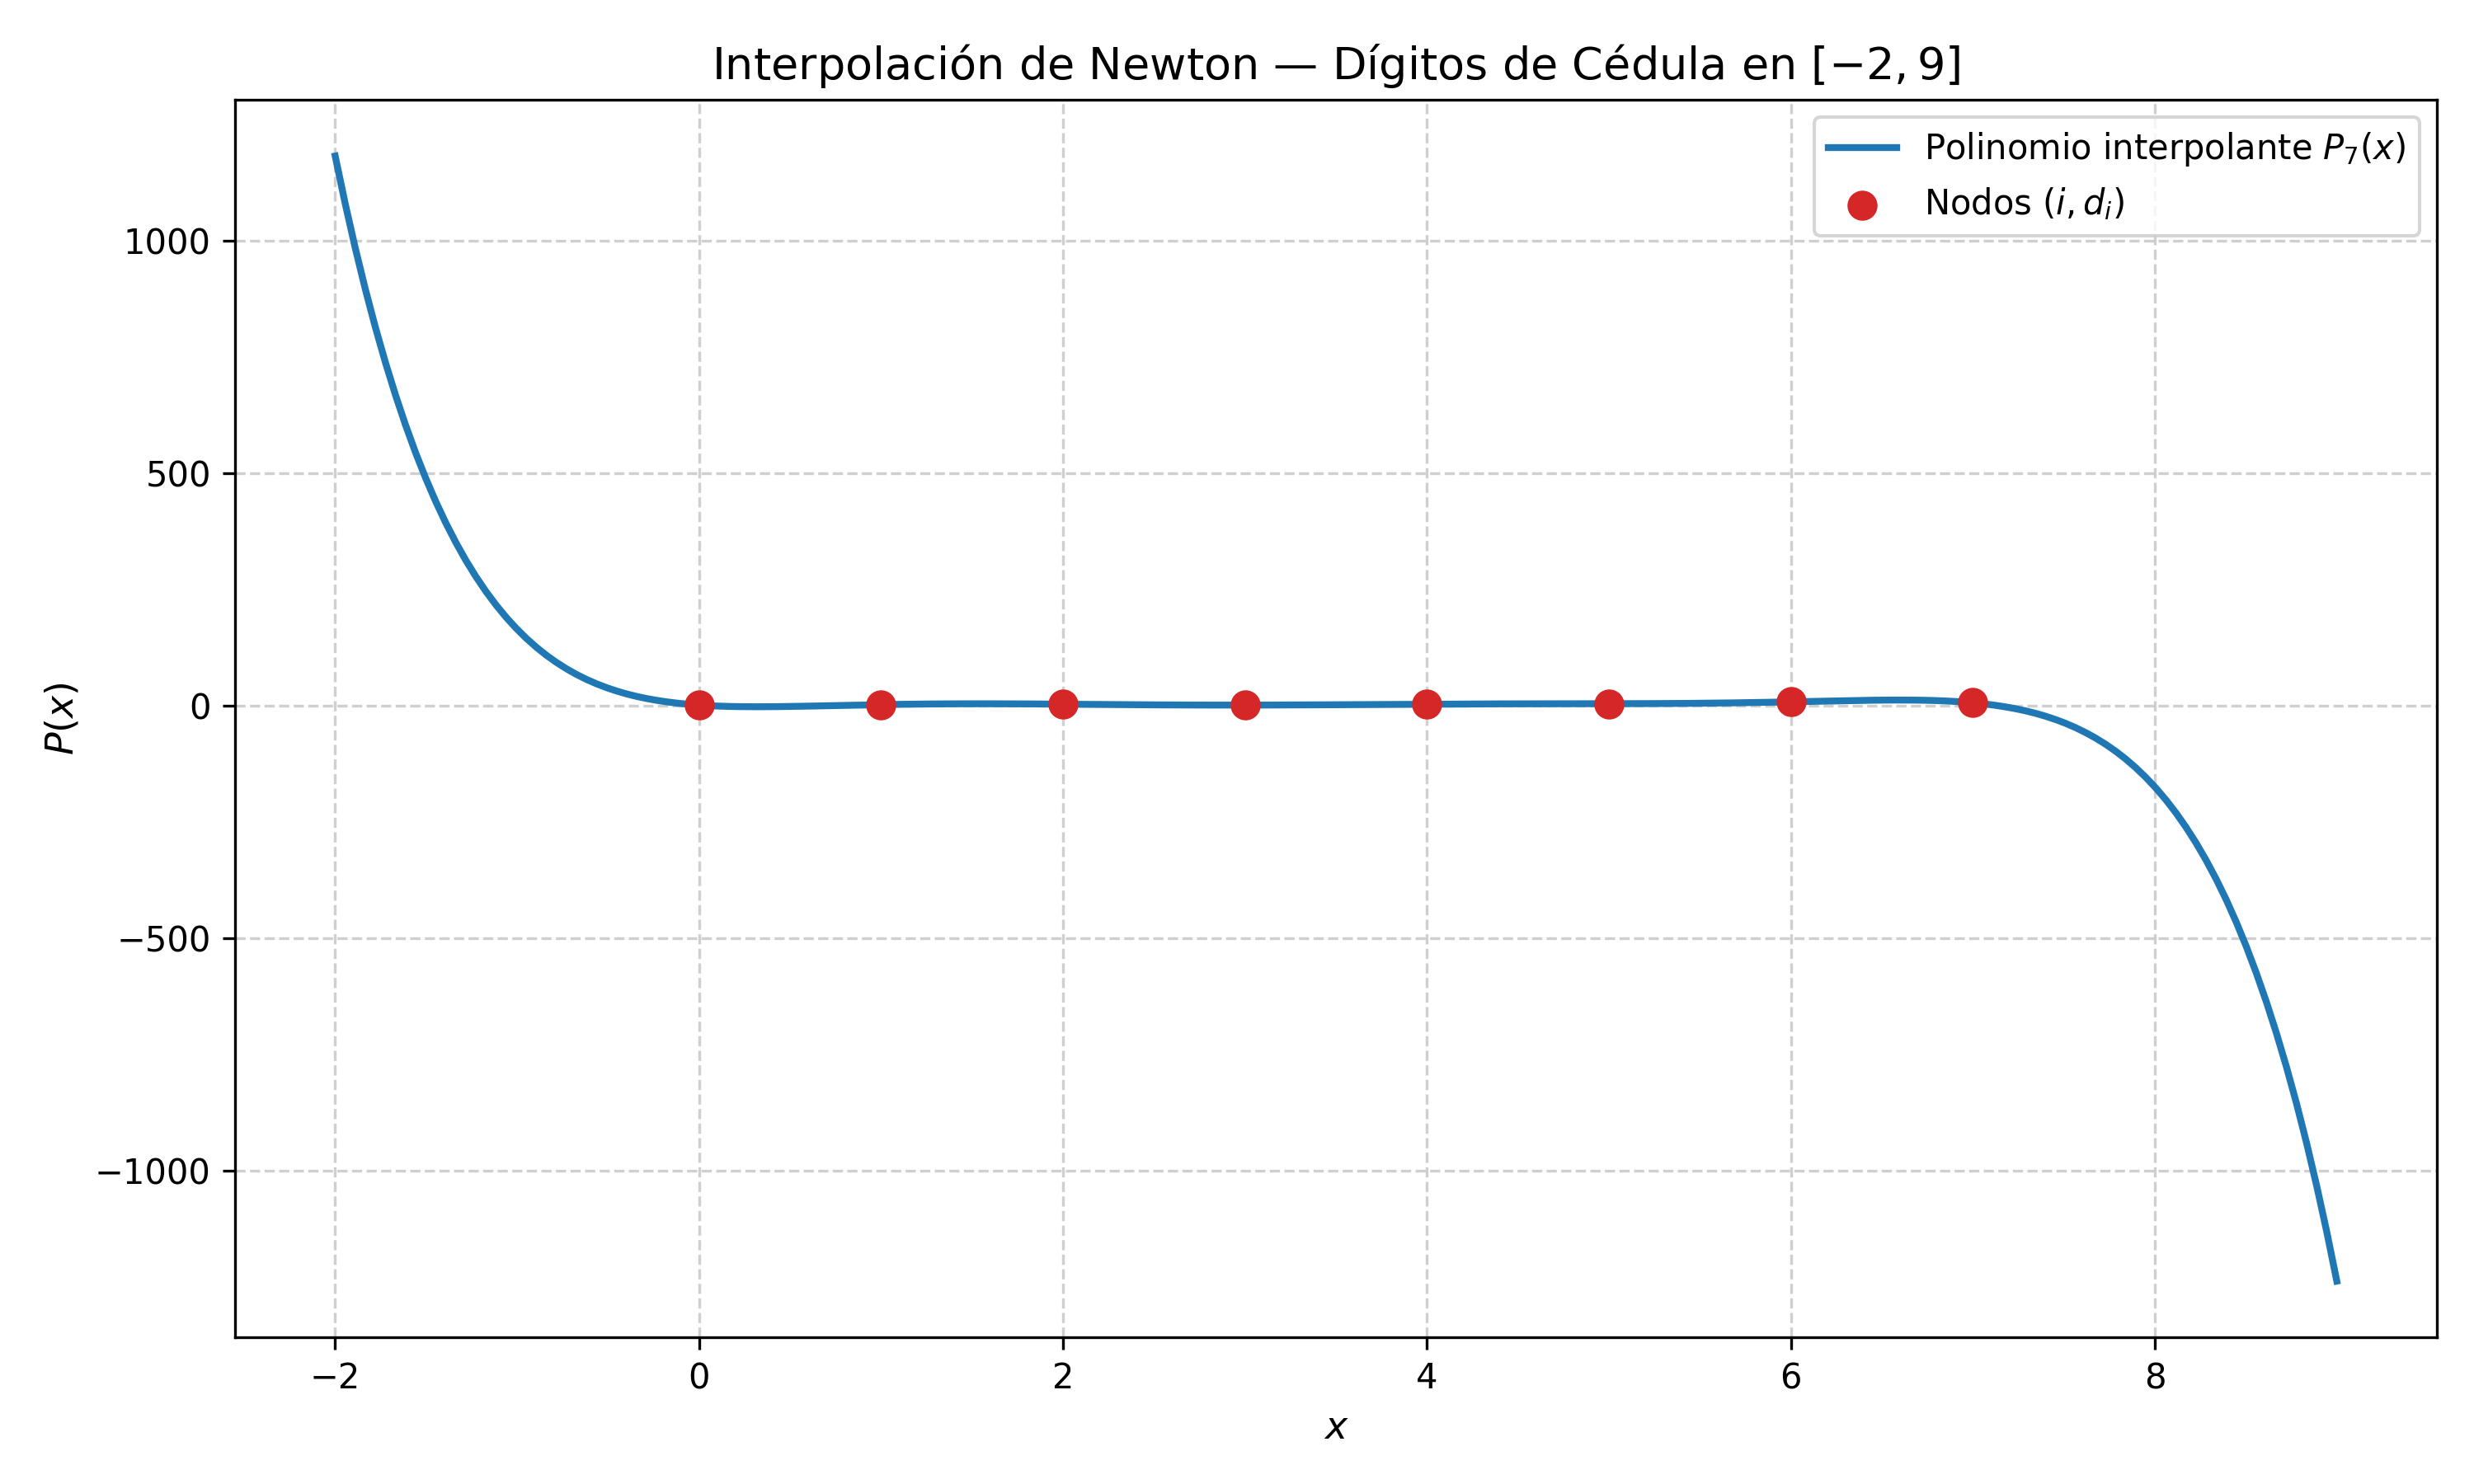
\includegraphics[width=0.84\textwidth]{p1_newton_cedula.png}
    \caption{Polinomio interpolante de Newton $P_7(x)$ evaluado en $[-2, 9]$ sobre los dígitos de la cédula 23.424.597.}
    \label{fig:p1_cedula}
\end{figure}

% ==================== PROBLEMA 2 ====================
\section{Problema 2: Aproximación Polinómica de Newton en $[-12, 12]$}

Considerando el último dígito de la cédula $d = 7$, el intervalo de trabajo es $[-(7+5),\, 7+5] = [-12, 12]$, y las dos funciones objetivo a aproximar mediante $n+1$ nodos equiespaciados para $n \in \{4, 7, 10\}$ son:
\begin{equation}
    f(x) = \frac{1}{1 + \left(\frac{5x}{12}\right)^2}, \qquad g(x) = \frac{1 + \cos\left(\frac{\pi x}{12}\right)}{2}.
\end{equation}

\subsection{Coeficientes de los Polinomios Interpolantes $P_n(x)$}

\begin{table}[H]
    \centering
    \caption{Coeficientes $c_{0,i}$ de diferencias divididas de Newton para $f(x)$ y $g(x)$ con $n \in \{4, 7, 10\}$ en $[-12, 12]$.}
    \label{tab:p2_coeficientes}
    \small
    \begin{tabular}{c|rrr|rrr}
        \toprule
        \multirow{2}{*}{$i$} & \multicolumn{3}{c|}{Función $f(x)$ (Tipo Runge)} & \multicolumn{3}{c}{Función $g(x)$ (Cosenoidal suave)} \\
        \cmidrule(lr){2-4} \cmidrule(lr){5-7}
         & $n = 4$ & $n = 7$ & $n = 10$ & $n = 4$ & $n = 7$ & $n = 10$ \\
        \midrule
        $0$  & $3.846154\times 10^{-2}$ & $3.846154\times 10^{-2}$ & $3.846154\times 10^{-2}$ & $0.000000\times 10^{0}$  & $0.000000\times 10^{0}$  & $0.000000\times 10^{0}$ \\
        $1$  & $1.657825\times 10^{-2}$ & $9.986305\times 10^{-3}$ & $8.484163\times 10^{-3}$ & $8.333333\times 10^{-2}$ & $5.490774\times 10^{-2}$ & $3.978813\times 10^{-2}$ \\
        $2$  & $1.059166\times 10^{-2}$ & $3.057951\times 10^{-3}$ & $1.806813\times 10^{-3}$ & $0.000000\times 10^{0}$  & $9.985038\times 10^{-3}$ & $1.341220\times 10^{-2}$ \\
        $3$  & $-1.918779\times 10^{-3}$ & $1.262535\times 10^{-3}$ & $4.582495\times 10^{-4}$ & $-7.716049\times 10^{-4}$ & $-1.317231\times 10^{-3}$ & $-1.151277\times 10^{-3}$ \\
        $4$  & $1.598982\times 10^{-4}$ & $-3.515381\times 10^{-4}$ & $1.295646\times 10^{-4}$ & $6.430041\times 10^{-5}$ & $1.902350\times 10^{-5}$ & $-2.831040\times 10^{-5}$ \\
        $5$  & --- & $3.564260\times 10^{-5}$ & $-2.557200\times 10^{-5}$ & --- & $3.383400\times 10^{-6}$ & $4.718400\times 10^{-6}$ \\
        $6$  & --- & $-1.732600\times 10^{-6}$ & $-5.919400\times 10^{-6}$ & --- & $-1.645000\times 10^{-7}$ & $-6.260000\times 10^{-8}$ \\
        $7$  & --- & $-3.394589\times 10^{-22}$ & $2.367800\times 10^{-6}$ & --- & $-2.117582\times 10^{-22}$ & $-6.000000\times 10^{-9}$ \\
        $8$  & --- & --- & $-3.905000\times 10^{-7}$ & --- & --- & $2.000000\times 10^{-10}$ \\
        $9$  & --- & --- & $4.280000\times 10^{-8}$ & --- & --- & $1.410000\times 10^{-11}$ \\
        $10$ & --- & --- & $-3.600000\times 10^{-9}$ & --- & --- & $-3.600000\times 10^{-12}$ \\
        \bottomrule
    \end{tabular}
\end{table}

\textit{Nota:} Para $n=7$ ($8$ nodos simétricos respecto a $x=0$), tanto $f(x)$ como $g(x)$ son funciones pares, por lo que la séptima diferencia dividida teórica es exactamente nula ($c_{0,7} \approx 0$ dentro de la precisión de punto flotante IEEE 754).

\subsection{Análisis de Convergencia y Fenómeno de Runge}
Al comparar ambas gráficas en la Figura~\ref{fig:p2_newton}, se observa una diferencia fundamental en la estabilidad de la interpolación global con nodos equiespaciados:
\begin{itemize}
    \item \textbf{Función $f(x)$ (Fenómeno de Runge):} Aunque $f(x) \in C^\infty[-12, 12]$, posee polos complejos conjugados cercanos al eje real en $z = \pm \frac{12}{5}i = \pm 2.4i$, dentro de la región de divergencia asociada a nodos equidistantes en $[-12, 12]$. En consecuencia, al aumentar el grado de $n=4$ a $n=7$ y $n=10$, el error máximo $\|f - P_n\|_\infty$ \textbf{diverge} cerca de los bordes $x = \pm 12$, produciendo oscilaciones violentas de amplitud creciente.
    \item \textbf{Función $g(x)$ (Convergencia uniforme):} Dado que $g(x)$ es una función entera (analítica en todo el plano complejo $\mathbb{C}$), sus derivadas de orden superior están uniformemente acotadas ($\|g^{(n+1)}\|_\infty \le \frac{1}{2}(\pi/12)^{n+1}$). Por ello, el término de error de Cauchy $\frac{g^{(n+1)}(\xi)}{(n+1)!}\prod_{k=0}^n(x-x_k)$ tiende rápidamente a cero: ya para $n=7$, $P_7(x)$ es visualmente indistinguible de $g(x)$ en todo $[-12, 12]$, y para $n=10$ el error es despreciable.
\end{itemize}

\begin{figure}[H]
    \centering
    \begin{subfigure}[b]{\textwidth}
        \centering
        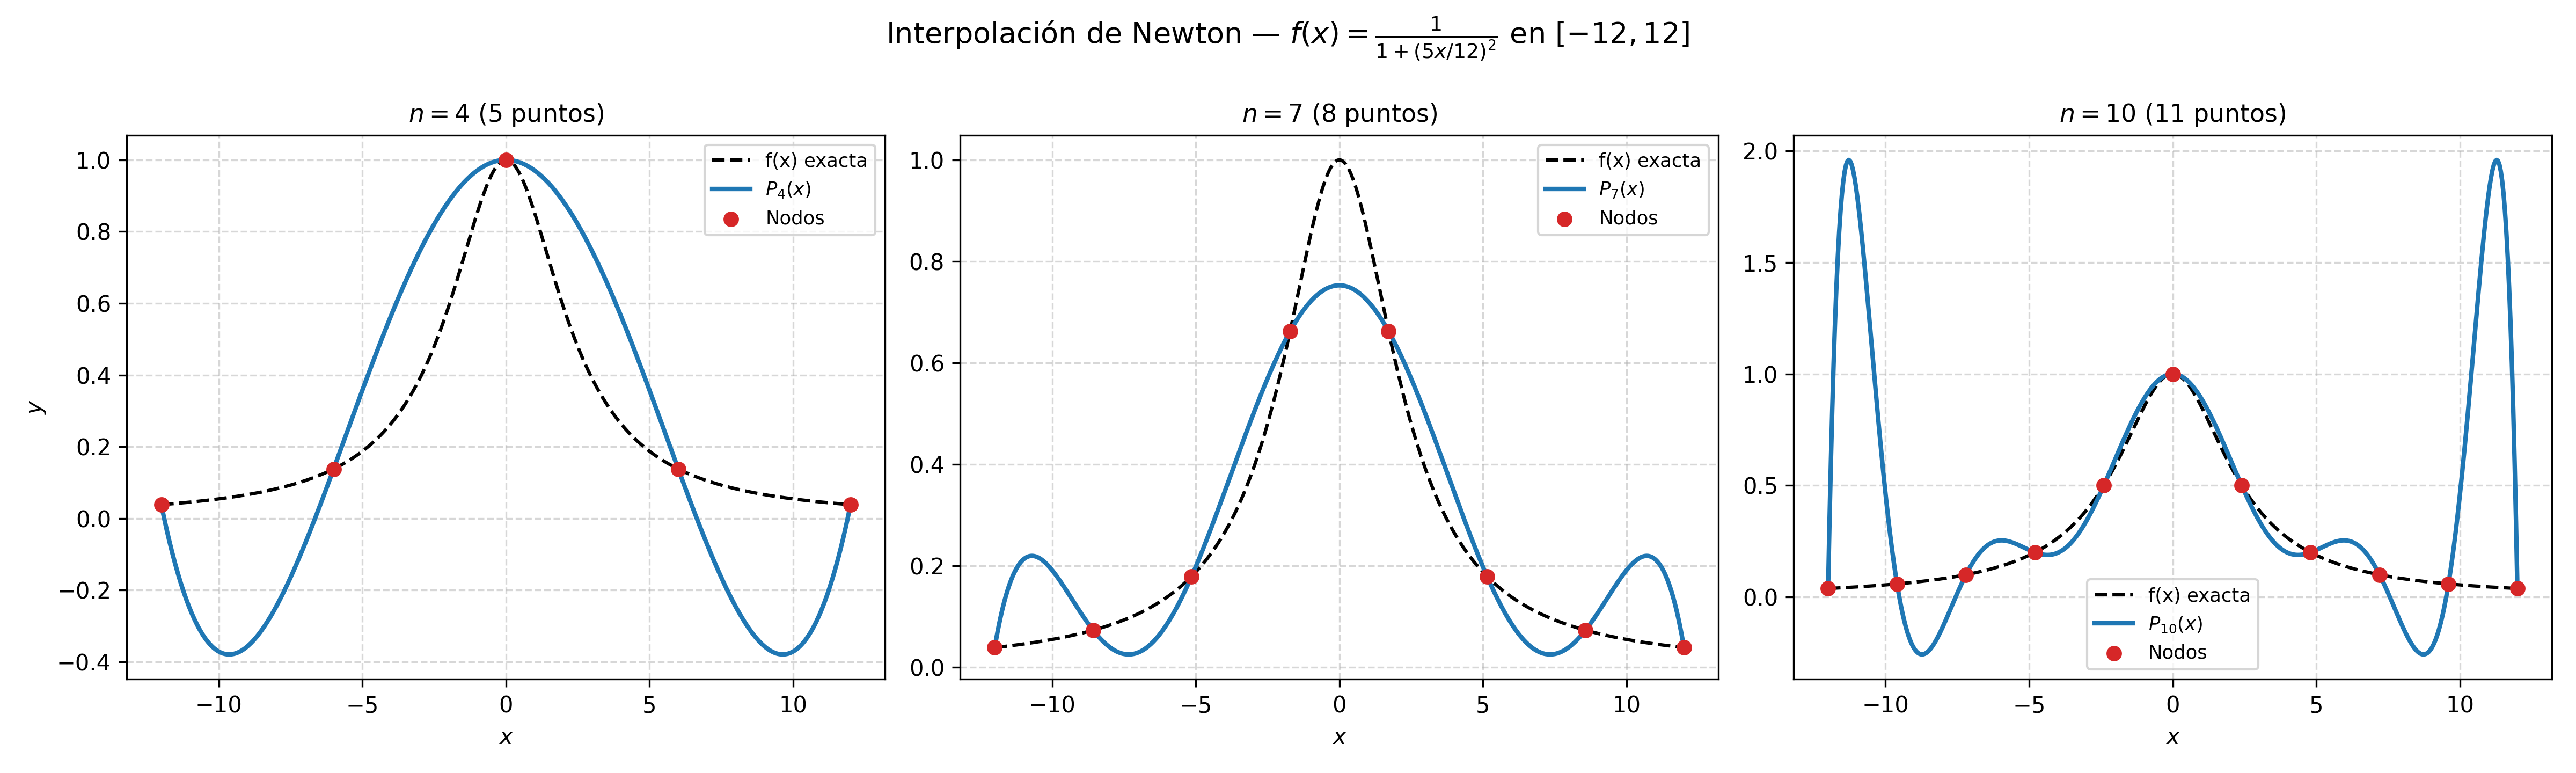
\includegraphics[width=\textwidth]{p2_newton_fx.png}
        \caption{Aproximación polinómica de Newton para $f(x)$: aparición del fenómeno de Runge en los extremos.}
    \end{subfigure}
    \vspace{0.35cm}
    \begin{subfigure}[b]{\textwidth}
        \centering
        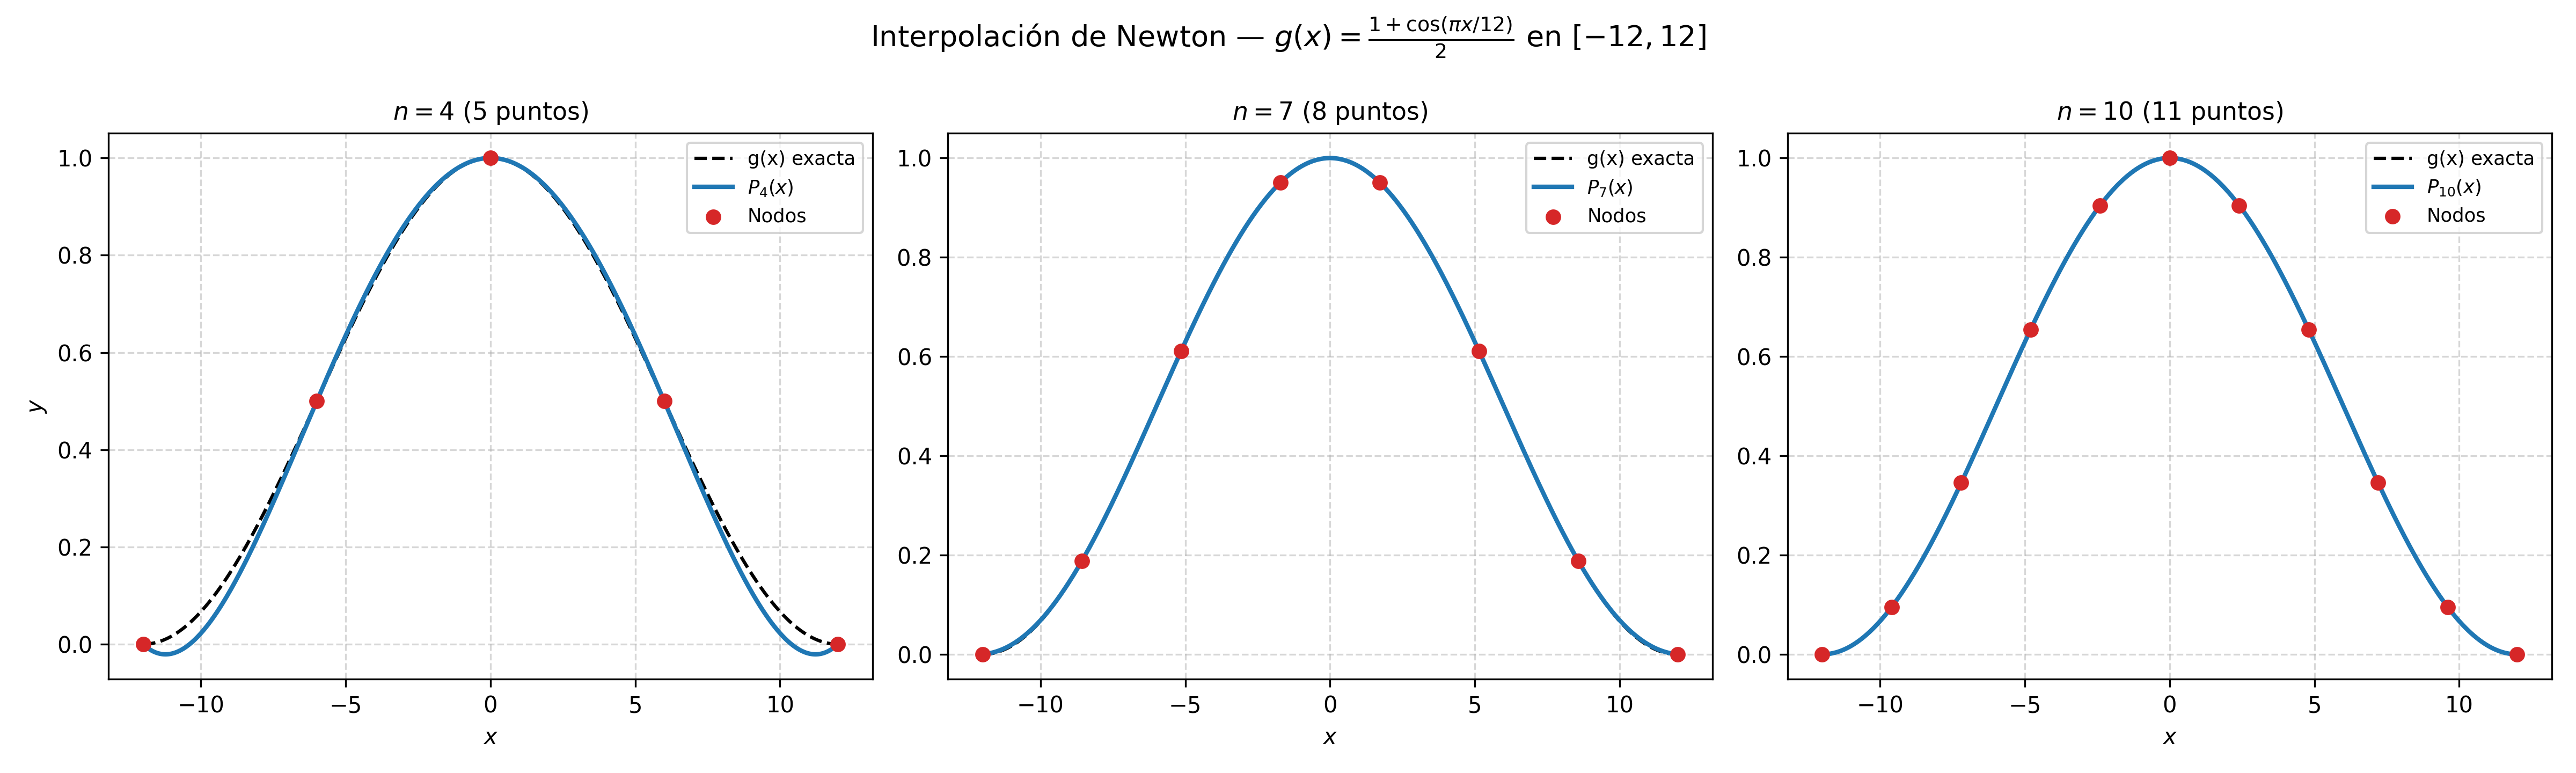
\includegraphics[width=\textwidth]{p2_newton_gx.png}
        \caption{Aproximación polinómica de Newton para $g(x)$: convergencia rápida y libre de oscilaciones.}
    \end{subfigure}
    \caption{Comparación de los polinomios interpolantes de Newton $P_n(x)$ ($n = 4, 7, 10$) en $[-12, 12]$.}
    \label{fig:p2_newton}
\end{figure}

% ==================== PROBLEMA 3 ====================
\section{Problema 3: Aproximación con Splines Cúbicos Naturales en $[-12, 12]$}

Para superar las oscilaciones globales observadas en $f(x)$, se aplicó el spline cúbico natural $S_j(x) = a_j + b_j(x-x_j) + c_j(x-x_j)^2 + d_j(x-x_j)^3$ sobre los mismos conjuntos de nodos equiespaciados ($n = 4, 7, 10$ tramos).

\subsection{Tablas de Coeficientes por Tramos}
Por su extensión, se presentan de forma íntegra los coeficientes obtenidos para $n=4$ y $n=10$ en ambas funciones (verificando en todos los casos la condición natural $c_0 = 0$, así como la simetría par respecto a $x=0$; los valores completos para $n=7$ constan en el archivo \texttt{resultados/p3\_coeficientes.txt}).

\begin{table}[H]
    \centering
    \caption{Coeficientes del Spline Cúbico Natural para $f(x)$ con $n = 4$ y $n = 10$ tramos en $[-12, 12]$.}
    \label{tab:p3_fx}
    \small
    \begin{tabular}{c|rrrrr}
        \toprule
        Tramo $j$ & $x_j$ & $a_j$ & $b_j$ & $c_j$ & $d_j$ \\
        \midrule
        \multicolumn{6}{c}{\textbf{$n = 4$ ($5$ nodos, $h = 6.0$)}} \\
        \midrule
        $0$ & $-12.0000$ & $0.03846154$ & $-0.04026146$ & $0.00000000$ & $0.00157888$ \\
        $1$ & $-6.0000$  & $0.13793103$ & $0.13025767$  & $0.02841986$ & $-0.00436385$ \\
        $2$ & $0.0000$   & $1.00000000$ & $0.00000000$  & $-0.05012947$ & $0.00436385$ \\
        $3$ & $6.0000$   & $0.13793103$ & $-0.13025767$ & $0.02841986$ & $-0.00157888$ \\
        \midrule
        \multicolumn{6}{c}{\textbf{$n = 10$ ($11$ nodos, $h = 2.4$)}} \\
        \midrule
        $0$ & $-12.0000$ & $0.03846154$ & $0.00734513$  & $0.00000000$  & $0.00019775$ \\
        $1$ & $-9.6000$  & $0.05882353$ & $0.01076223$  & $0.00142379$  & $0.00051693$ \\
        $2$ & $-7.2000$  & $0.10000000$ & $0.02652902$  & $0.00514570$  & $0.00048402$ \\
        $3$ & $-4.8000$  & $0.20000000$ & $0.05959226$  & $0.00863064$  & $0.00775941$ \\
        $4$ & $-2.4000$  & $0.50000000$ & $0.23510193$  & $0.06449839$  & $-0.03152165$ \\
        $5$ & $0.0000$   & $1.00000000$ & $0.00000000$  & $-0.16245753$ & $0.03152165$ \\
        $6$ & $2.4000$   & $0.50000000$ & $-0.23510193$ & $0.06449839$  & $-0.00775941$ \\
        $7$ & $4.8000$   & $0.20000000$ & $-0.05959226$ & $0.00863064$  & $-0.00048402$ \\
        $8$ & $7.2000$   & $0.10000000$ & $-0.02652902$ & $0.00514570$  & $-0.00051693$ \\
        $9$ & $9.6000$   & $0.05882353$ & $-0.01076223$ & $0.00142379$  & $-0.00019775$ \\
        \bottomrule
    \end{tabular}
\end{table}

\begin{table}[H]
    \centering
    \caption{Coeficientes del Spline Cúbico Natural para $g(x)$ con $n = 4$ y $n = 10$ tramos en $[-12, 12]$.}
    \label{tab:p3_gx}
    \small
    \begin{tabular}{c|rrrrr}
        \toprule
        Tramo $j$ & $x_j$ & $a_j$ & $b_j$ & $c_j$ & $d_j$ \\
        \midrule
        \multicolumn{6}{c}{\textbf{$n = 4$ ($5$ nodos, $h = 6.0$)}} \\
        \midrule
        $0$ & $-12.0000$ & $0.00000000$ & $0.07142857$  & $0.00000000$  & $0.00033069$ \\
        $1$ & $-6.0000$  & $0.50000000$ & $0.10714286$  & $0.00595238$  & $-0.00165344$ \\
        $2$ & $0.0000$   & $1.00000000$ & $0.00000000$  & $-0.02380952$ & $0.00165344$ \\
        $3$ & $6.0000$   & $0.50000000$ & $-0.10714286$ & $0.00595238$  & $-0.00033069$ \\
        \midrule
        \multicolumn{6}{c}{\textbf{$n = 10$ ($11$ nodos, $h = 2.4$)}} \\
        \midrule
        $0$ & $-12.0000$ & $0.00000000$ & $0.02453342$  & $0.00000000$  & $0.00264839$ \\
        $1$ & $-9.6000$  & $0.09549150$ & $0.07029754$  & $0.01906838$  & $-0.00206510$ \\
        $2$ & $-7.2000$  & $0.34549150$ & $0.12614080$  & $0.00419964$  & $-0.00129564$ \\
        $3$ & $-4.8000$  & $0.65450850$ & $0.12391049$  & $-0.00512894$ & $-0.00129069$ \\
        $4$ & $-2.4000$  & $0.90450850$ & $0.07698847$  & $-0.01442190$ & $-0.00044927$ \\
        $5$ & $0.0000$   & $1.00000000$ & $0.00000000$  & $-0.01765663$ & $0.00044927$ \\
        $6$ & $2.4000$   & $0.90450850$ & $-0.07698847$ & $-0.01442190$ & $0.00129069$ \\
        $7$ & $4.8000$   & $0.65450850$ & $-0.12391049$ & $-0.00512894$ & $0.00129564$ \\
        $8$ & $7.2000$   & $0.34549150$ & $-0.12614080$ & $0.00419964$  & $0.00206510$ \\
        $9$ & $9.6000$   & $0.09549150$ & $-0.07029754$ & $0.01906838$  & $-0.00264839$ \\
        \bottomrule
    \end{tabular}
\end{table}

\subsection{Comparación Crítica: Interpolación Global vs. Interpolación a Trozos}
Los resultados de la Figura~\ref{fig:p3_spline} confirman la superioridad numérica de los splines cúbicos frente a la interpolación polinómica de grado elevado:
\begin{enumerate}
    \item \textbf{Eliminación del fenómeno de Runge:} Al mantener fijo el grado cúbico ($3$) en cada subintervalo y refinar el tamaño de paso $h = 24/n$, el error satisface $\|f - S\|_\infty = \mathcal{O}(h^4)$ para funciones $C^4$. Para $n=10$ ($h=2.4$), $S_{10}(x)$ reproduce $f(x)$ con total fidelidad tanto en el pico central como en las colas laterales, sin inestabilidades.
    \item \textbf{Propiedad de mínima curvatura:} El spline cúbico natural minimiza la integral de energía de flexión $\int_{-12}^{12} [S''(x)]^2\,dx$ entre todas las funciones de clase $C^2$ que interpolan los nodos, evitando oscilaciones espurias entre puntos consecutivos.
\end{enumerate}

\begin{figure}[H]
    \centering
    \begin{subfigure}[b]{\textwidth}
        \centering
        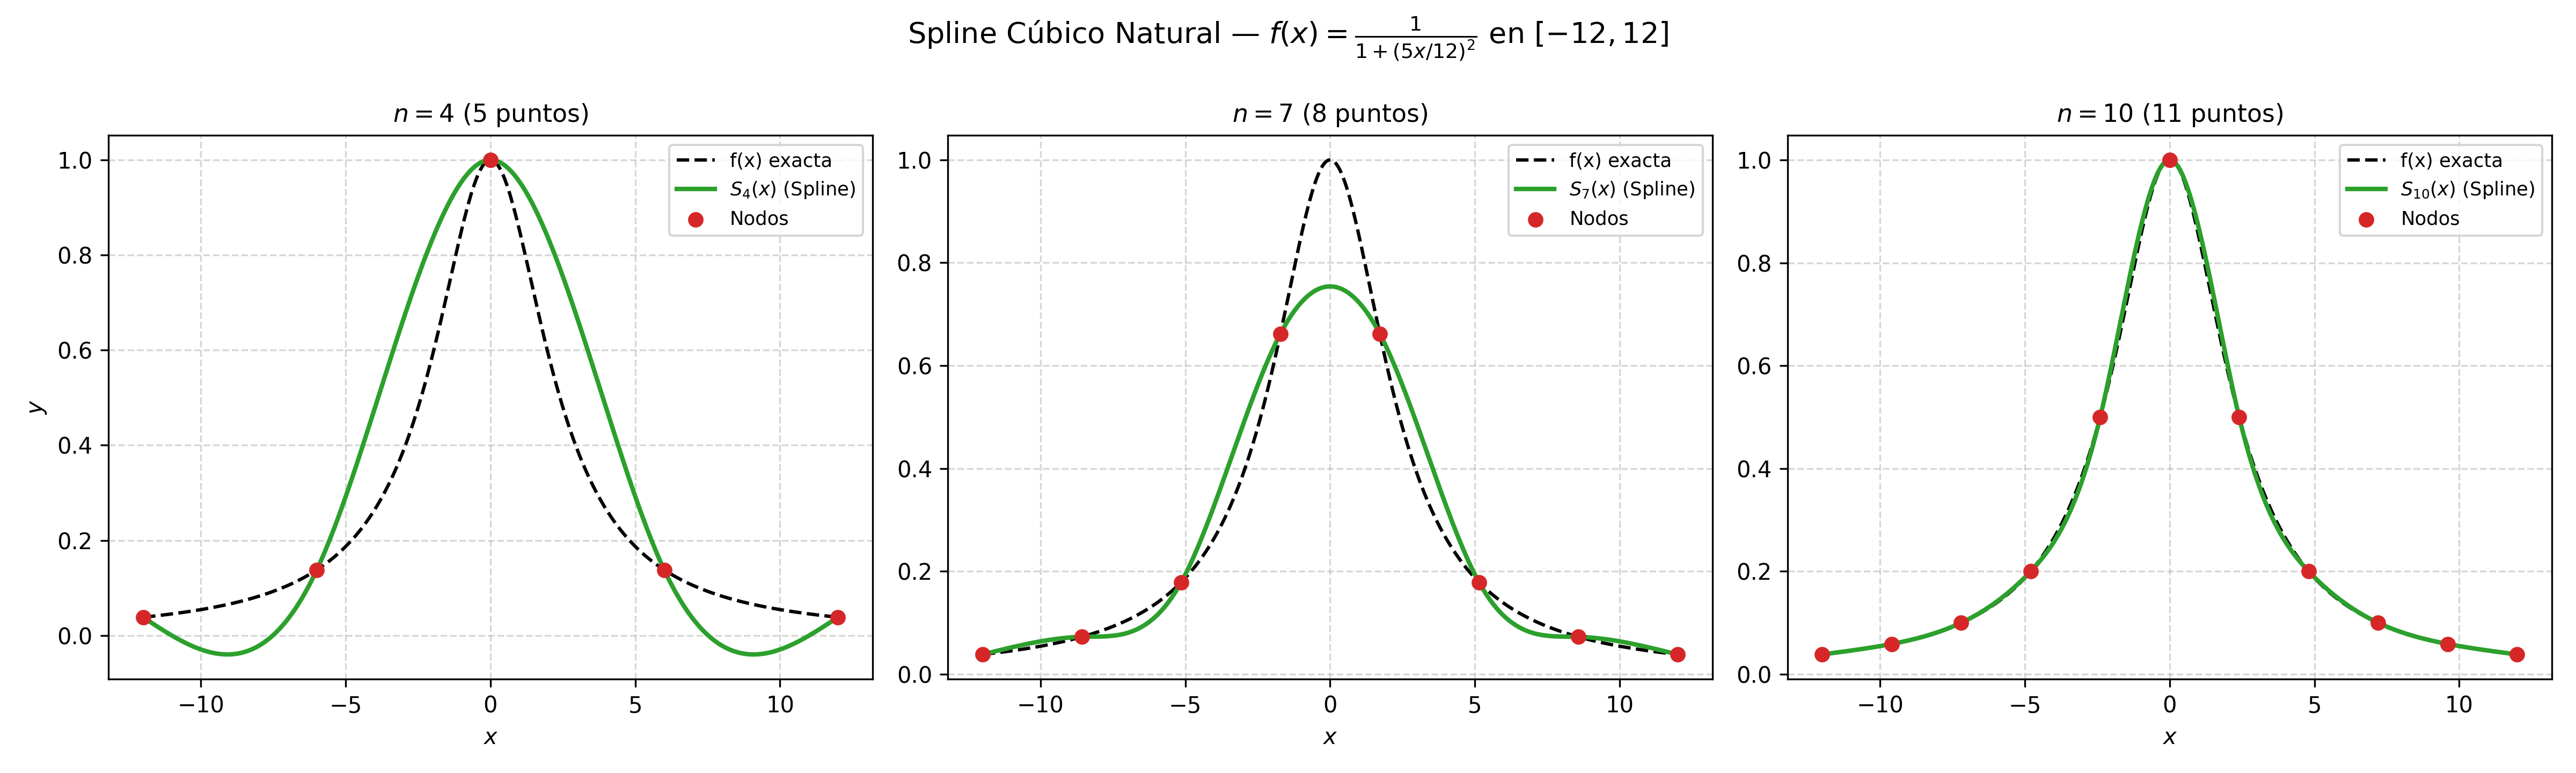
\includegraphics[width=\textwidth]{p3_spline_fx.png}
        \caption{Spline cúbico natural aplicado a $f(x)$: convergencia monótona sin oscilaciones de Runge.}
    \end{subfigure}
    \vspace{0.35cm}
    \begin{subfigure}[b]{\textwidth}
        \centering
        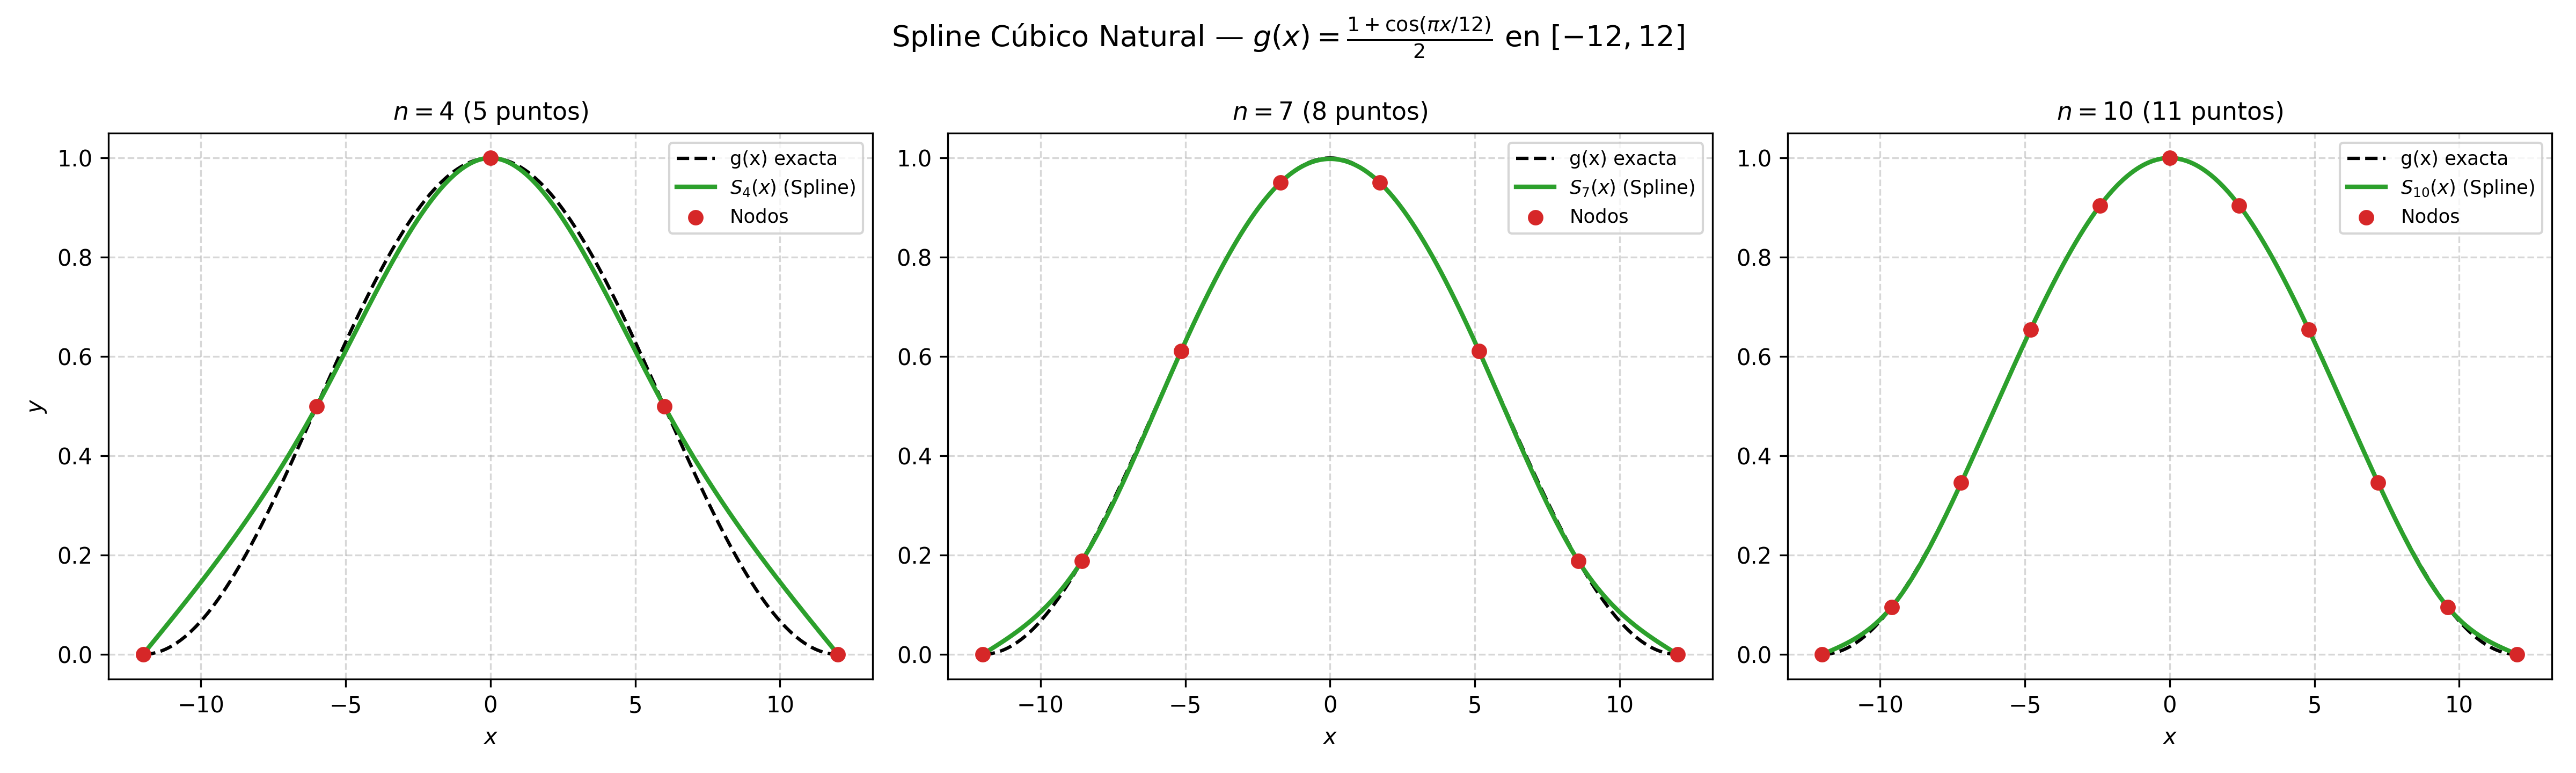
\includegraphics[width=\textwidth]{p3_spline_gx.png}
        \caption{Spline cúbico natural aplicado a $g(x)$: aproximación suave en todos los tramos.}
    \end{subfigure}
    \caption{Aproximación mediante Splines Cúbicos Naturales para $n \in \{4, 7, 10\}$ en $[-12, 12]$.}
    \label{fig:p3_spline}
\end{figure}

% ==================== PROBLEMA 4 ====================
\section{Problema 4: Modelado Paramétrico de Curva Plana (Inicial ``L'')}

\subsection{Metodología de Digitalización y Parametrización por Longitud de Arco}
Dado que la letra caligráfica \textbf{``L''} (en tipografía Old English cursiva) constituye una curva plana no funcional con auto-intersecciones y múltiples valores de $y$ para un mismo $x$, no puede representarse como $y = f(x)$. En su lugar, se discretizó el trazo continuo mediante $90$ puntos ordenados $(x_i, y_i)$ ($i = 0, \dots, 89$, equivalentes a $n = 89$ subintervalos) sobre un sistema de coordenadas normalizado $[0, 10] \times [0, 10]$.

Para evitar distorsiones por espaciamiento irregular de los clics, se asignó el parámetro $t_i$ mediante la \textbf{longitud acumulada de la poligonal}:
\begin{equation}
    t_0 = 0, \qquad t_i = t_{i-1} + \sqrt{(x_i - x_{i-1})^2 + (y_i - y_{i-1})^2}, \quad i = 1, \dots, 89,
\end{equation}
alcanzando una longitud de arco poligonal total $t_{89} = 43.974050$ unidades. A partir de la secuencia estrictamente creciente $\{t_i\}_{i=0}^{89}$, se construyeron dos splines cúbicos naturales independientes: $x(t) = S_x(t)$ interpolando $(t_i, x_i)$ y $y(t) = S_y(t)$ interpolando $(t_i, y_i)$.

\subsection{Muestra de Nodos y Coeficientes de $S_x(t)$ y $S_y(t)$}
La Tabla~\ref{tab:p4_muestra} recoge una selección representativa de los nodos iniciales, intermedios y finales junto con sus coeficientes cúbicos correspondientes (el listado completo de los $90$ nodos y $89$ tramos se encuentra en \texttt{resultados/p4\_coeficientes.txt}).

\begin{table}[H]
    \centering
    \caption{Muestra representativa de nodos $(t_i, x_i, y_i)$ y coeficientes de $S_x(t)$ y $S_y(t)$ para la inicial ``L'' ($90$ nodos, $89$ tramos).}
    \label{tab:p4_muestra}
    \scriptsize
    \begin{tabular}{c|rrr|rrrr|rrrr}
        \toprule
        \multirow{2}{*}{$j$} & \multirow{2}{*}{$t_j$} & \multirow{2}{*}{$x_j$} & \multirow{2}{*}{$y_j$} & \multicolumn{4}{c|}{Spline $S_x(t)$} & \multicolumn{4}{c}{Spline $S_y(t)$} \\
        \cmidrule(lr){5-8} \cmidrule(lr){9-12}
         & & & & $a_{x,j}$ & $b_{x,j}$ & $c_{x,j}$ & $d_{x,j}$ & $a_{y,j}$ & $b_{y,j}$ & $c_{y,j}$ & $d_{y,j}$ \\
        \midrule
        $0$  & $0.0000$  & $7.684$ & $4.479$ & $7.6840$ & $0.8740$  & $0.0000$  & $-0.1680$ & $4.4790$ & $0.4795$  & $0.0000$  & $0.3133$ \\
        $1$  & $0.4435$  & $8.057$ & $4.719$ & $8.0570$ & $0.7749$  & $-0.2235$ & $-0.4649$ & $4.7190$ & $0.6644$  & $0.4169$  & $-0.1335$ \\
        $17$ & $5.9400$  & $4.516$ & $4.695$ & $4.5160$ & $0.2812$  & $1.2151$  & $-0.7419$ & $4.6950$ & $-0.9738$ & $0.3337$  & $0.6624$ \\
        $28$ & $10.5601$ & $5.992$ & $6.796$ & $5.9920$ & $-1.0021$ & $-0.0196$ & $0.0678$  & $6.7960$ & $0.0952$  & $-0.1927$ & $-0.1699$ \\
        $35$ & $14.3961$ & $3.100$ & $4.707$ & $3.1000$ & $-0.0166$ & $0.5835$  & $-0.3582$ & $4.7070$ & $-0.9715$ & $0.0373$  & $-0.0976$ \\
        $52$ & $22.4791$ & $9.401$ & $5.536$ & $9.4010$ & $-0.9035$ & $-1.2185$ & $3.7917$  & $5.5360$ & $0.4087$  & $-2.7596$ & $2.7170$ \\
        $63$ & $26.6302$ & $9.629$ & $6.400$ & $9.6290$ & $-1.0508$ & $0.0422$  & $0.2039$  & $6.4000$ & $0.2509$  & $-0.6276$ & $-0.1446$ \\
        $78$ & $36.1933$ & $1.948$ & $2.091$ & $1.9480$ & $-0.5233$ & $2.1788$  & $-0.0752$ & $2.0910$ & $0.8396$  & $1.8865$  & $-5.3263$ \\
        $88$ & $43.7508$ & $8.849$ & $2.943$ & $8.8490$ & $0.8050$  & $0.0092$  & $-0.0137$ & $2.9430$ & $0.5925$  & $-0.0073$ & $0.0110$ \\
        \bottomrule
    \end{tabular}
\end{table}

\subsection{Evaluación Gráfica de la Reconstrucción}
Evaluando $(S_x(t), S_y(t))$ sobre una malla fina de $1000$ valores en $[0, 43.974050]$, se obtiene la curva mostrada en la Figura~\ref{fig:p4_letra}. La superposición sobre la tipografía de referencia demuestra que la parametrización por longitud de arco combinada con una alta densidad de puntos ($90$ nodos) en los rizos de mayor curvatura captura con precisión tanto las espirales internas como los lazos inferiores, garantizando continuidad geométrica $G^2$ sin sobreimpulsos artificiales.

\begin{figure}[H]
    \centering
    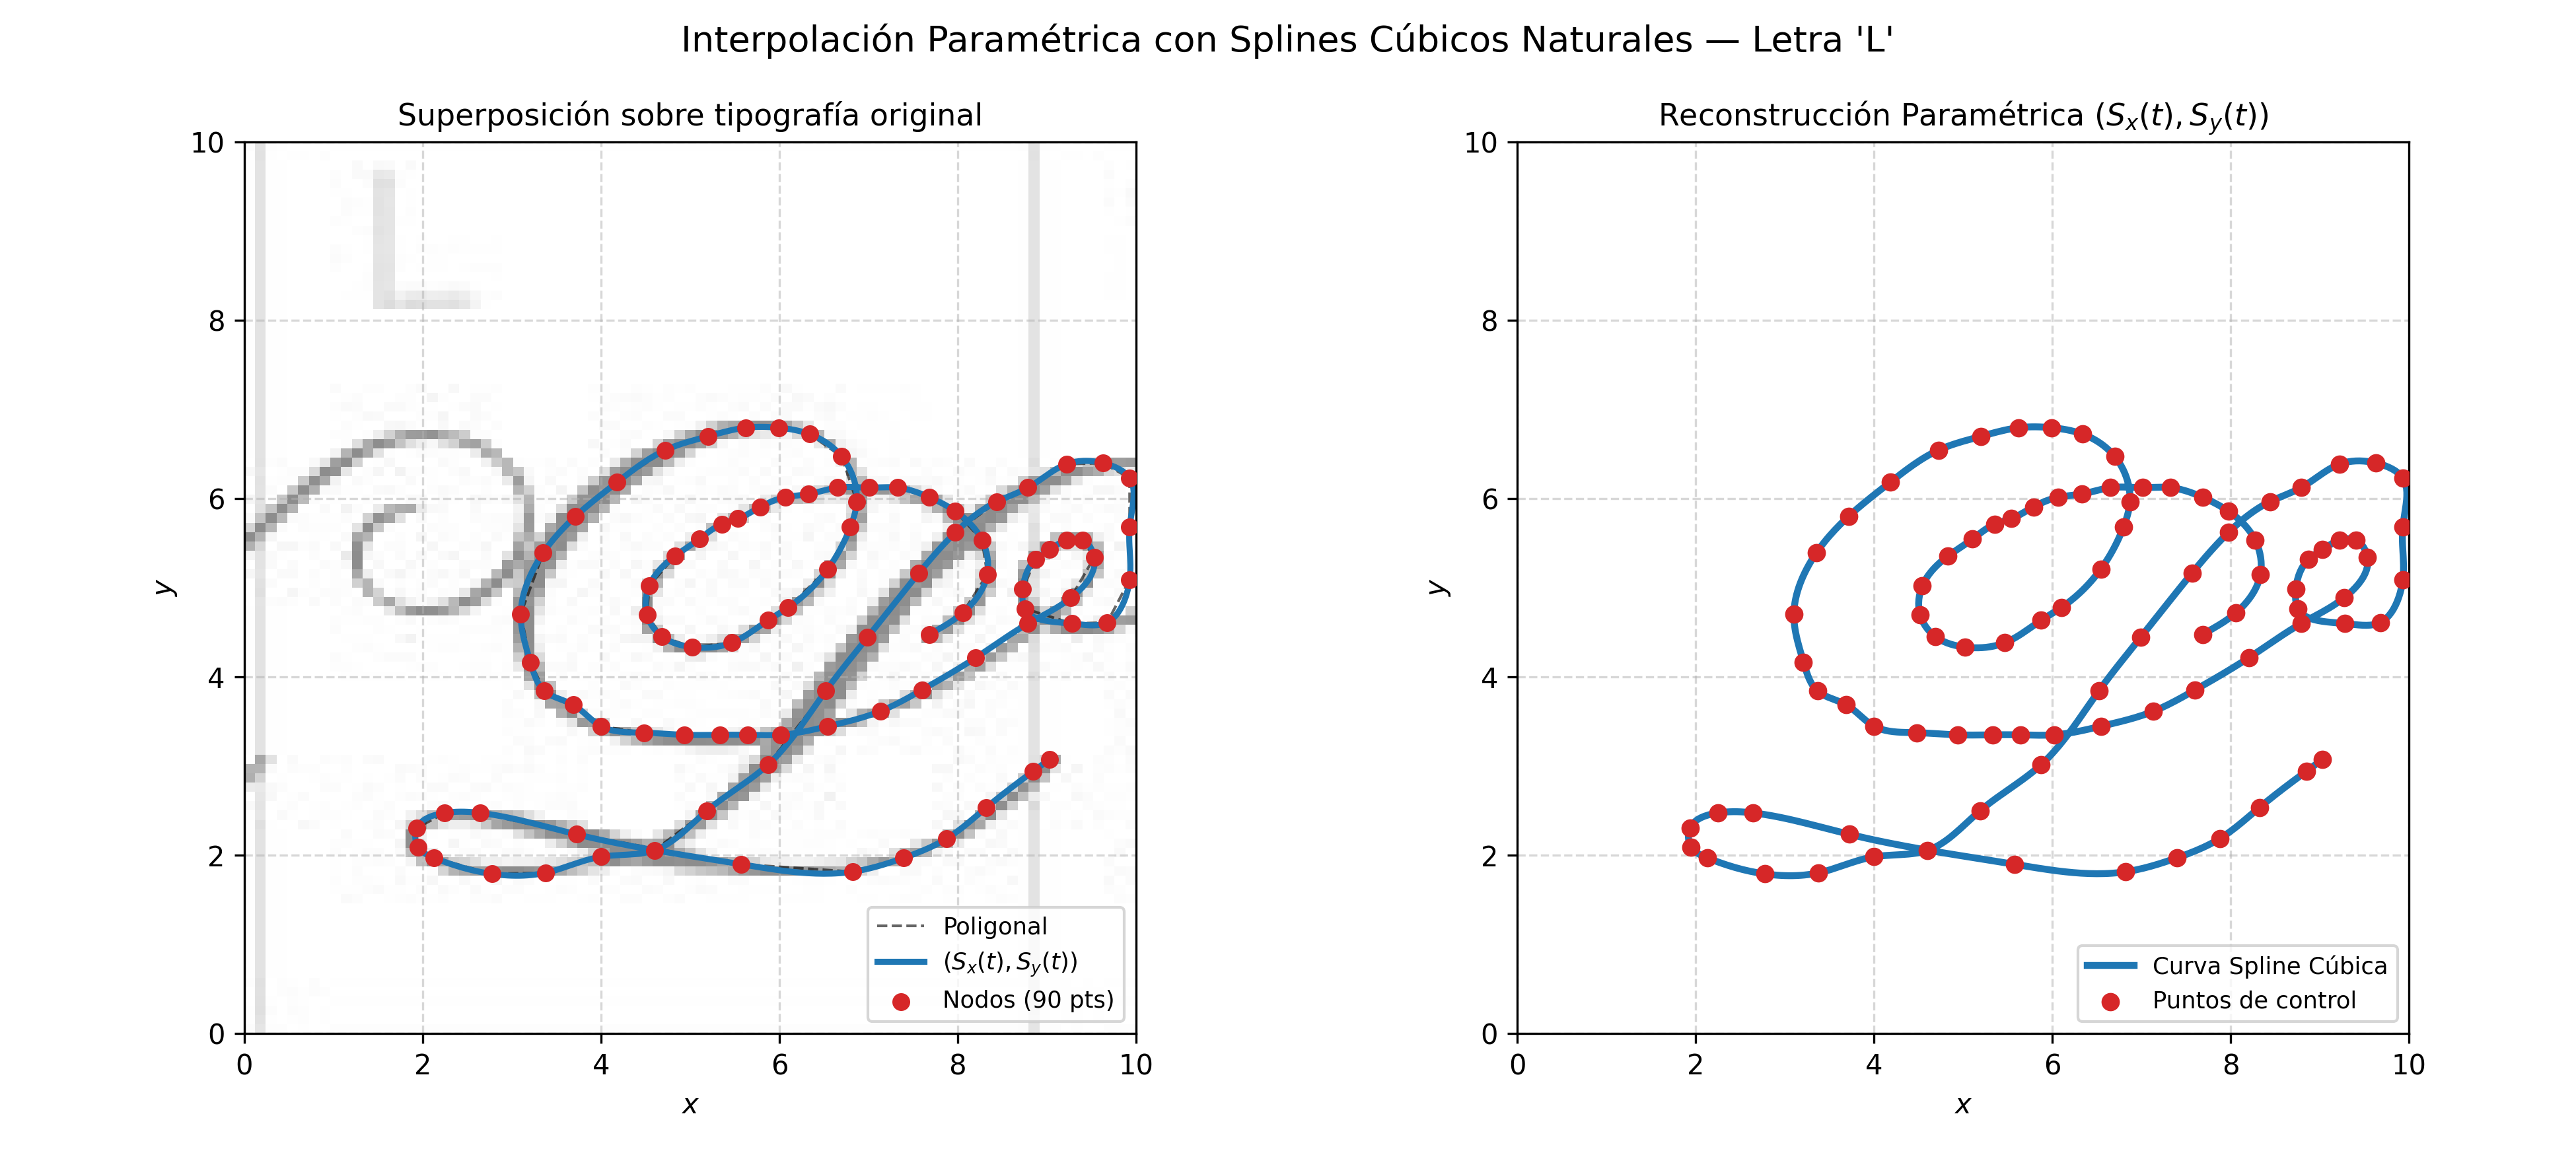
\includegraphics[width=\textwidth]{p4_letra_parametrica.png}
    \caption{Superposición sobre la tipografía original (izquierda) y reconstrucción paramétrica limpia $(S_x(t), S_y(t))$ de la inicial ``L'' mediante splines cúbicos naturales (derecha).}
    \label{fig:p4_letra}
\end{figure}

% ==================== CONCLUSIONES ====================
\section{Conclusiones}
\begin{enumerate}
    \item \textbf{Sensibilidad a la extrapolación y al grado polinómico:} En el Problema~1 se comprobó que el polinomio de grado $7$ interpola exactamente los dígitos de la cédula en $[0, 7]$, pero diverge rápidamente fuera de dicho dominio. En el Problema~2 se evidenció que el éxito de la interpolación global sobre nodos equiespaciados depende de la analiticidad de la función: mientras $g(x)$ converge suavemente al aumentar $n$, $f(x)$ exhibe el fenómeno de Runge cerca de $x = \pm 12$.
    \item \textbf{Estabilidad de los splines cúbicos naturales:} La interpolación segmentaria de grado $3$ con continuidad $C^2$ (Problema~3) elimina por completo las oscilaciones de Runge en $f(x)$ y garantiza convergencia uniforme al reducir el paso $h$.
    \item \textbf{Versatilidad en diseño geométrico (CAD/tipografía):} La parametrización por longitud de arco acumulada $t_i$ convierte curvas planas cerradas o con múltiples vueltas en dos problemas escalares unidimensionales suaves $(S_x(t), S_y(t))$, permitiendo reconstruir fielmente la inicial caligráfica ``L''.
\end{enumerate}

\end{document}